
\chapter{Estimate Fusion on an Untrusted Cloud}\label{ch:cloud_fusion}

% 
% 8888888b.  8888888b.   .d88888b.  888888b.   
% 888   Y88b 888   Y88b d88P" "Y88b 888  "88b  
% 888    888 888    888 888     888 888  .88P  
% 888   d88P 888   d88P 888     888 8888888K.  
% 8888888P"  8888888P"  888     888 888  "Y88b 
% 888        888 T88b   888     888 888    888 
% 888        888  T88b  Y88b. .d88P 888   d88P 
% 888        888   T88b  "Y88888P"  8888888P"  
%                                              
%                                              
%                                              
% 

\section{Problem Formulation}\label{sec:cloud_fusion:problem}
Motivated by the key step in multi-sensor fusion, we are interested in transmitting local sensor state estimate and covariance information over a network to be fused by a fusion cloud. In particular, we consider centralised FCI fusion, as introduced in section \ref{subsec:prelims:fci}, over a public network and at an untrusted fusion cloud. The aim is for fusion to be computed by the cloud on encrypted sensor data to preserve individual and fused estimate confidentiality, that is, no estimate information should be made available to network eavesdroppers, sensors that did not produce it or the fusion cloud itself. A trusted querying third party, holding appropriate secret keys, is presumed to exist which can request and process the fused estimate information from the cloud.

The concrete estimation problem is captured by a time-independent process defined by its state $\vec{x} \in \mathbb{R}^d$ and is estimated by sensors $i$, $1\leq i\leq n$, each producing a state estimate and estimate error covariance,
\begin{equation}
    \hat{\vec{x}}_i \in \mathbb{R}^d \text{ and } \mat{P}_i \in \mathbb{R}^{d\times d}\,,
\end{equation}
respectively. As we are interested in computing the FCI algorithm, we consider sensors that produce estimates in the information form, namely, the information vector and information matrix,
\begin{equation}\label{eq:cloud_fusion:sen_info_vecs_and_mats}
    \mat{P}_i^{-1}\hat{\vec{x}}_i \text{ and } \mat{P}_i^{-1}\,,
\end{equation}
instead. Information \eqref{eq:cloud_fusion:sen_info_vecs_and_mats} is to be sent to the fusion cloud where FCI is computed and a fused information vector and information matrix,
\begin{equation}\label{eq:cloud_fusion:fus_info_vec_and_mat}
    \mat{P}_{\mathsf{fus}}^{-1}\hat{\vec{x}}_{\mathsf{fus}} \in \mathbb{R}^d \text{ and } \mat{P}_{\mathsf{fus}}^{-1} \in \mathbb{R}^{d\times d}\,,
\end{equation}
are produced. A trusted querying party can then request \eqref{eq:cloud_fusion:fus_info_vec_and_mat} from the cloud when desired.

The cryptographic aims of this problem are captured by the actions of the involved parties and the accepted leakage of confidential information. 
\begin{description}
    \item[Honest-but-curious parties] We assume that all sensors and the fusion cloud follow fusion protocols correctly and that no injection or modification to transmitted data is performed by network eavesdroppers, but all parties may use any learned information for external malicious gain. Collusion between any malicious parties is considered possible.
    \item[Encrypted estimates meeting IND-CPA] Permitted leakage is such that all estimate information available to a colluding subset of malicious parties, excluding any locally produced estimates (in the case of malicious sensors), is encrypted with a scheme meeting the IND-CPA cryptographic notion, introduced in section \ref{subsec:prelims:crypto_notions}.
\end{description}

The relatively strict estimation and security aims above can be difficult to achieve in general and relaxations of some requirements may be necessary to achieve others. This will be seen in the two methods presented later in this chapter. Participants, communications between them and whether they are trusted, concerning the ideal aims above, are summarised graphically in figure \ref{fig:cloud_fusion:problem_layout}.
\begin{figure}[htbp]
    \centering
    \begin{tikzpicture}
        % Estimators
        \fill [pyplotred!70] (1.4,5.75) rectangle (3.6,5.25);
        \fill [pyplotred!70] (5.9,5.75) rectangle (8.1,5.25);
        \node at (2.5,5.5) {Estimator $1$};
        \node at (7,5.5) {Estimator $n$};
        % Dots
        \fill [black] (5,5.5) circle (0.05);
        \fill [black] (4.5,5.5) circle (0.05);
        \fill [black] (4.75,5.5) circle (0.05);
        % Estimates
        \node [left] at (3.25,4.25) {$\mat{P}_1^{-1}\hat{\vec{x}}_1,\mat{P}_1^{-1}$};
        \node [right] at (6.25,4.25) {$\mat{P}_n^{-1}\hat{\vec{x}}_n,\mat{P}_n^{-1}$};
        % Estimator arrows
        \draw [-latex]  plot coordinates {(3,5)  (4.25,2.75)};
        \draw [-latex]  plot coordinates {(6.5,5)  (5.25,2.75)};
        % Network
        \fill [pyplotred!70] (2.65,3.75) rectangle (6.85,3.25);
        \node at (4.75,3.5) {Network Eavesdroppers};
        % Cloud
        \fill [pyplotred!70] (4.6,2.35) ellipse (0.5 and 0.4);
        \fill [pyplotred!70] (5.25,2.1) ellipse (0.25 and 0.25);
        \fill [pyplotred!70] (4.25,2.1) ellipse (0.25 and 0.25);
        \fill [pyplotred!70] (5.1,2.35) ellipse (0.25 and 0.25);
        \fill [pyplotred!70] (4.25,1.85) rectangle (5.25,2.1);
        \node at (4.75,2.15) {Cloud};
         % Fusion
        \node [right] at (4.75,1.25) {$\mat{P}_{\mathsf{fus}}^{-1}\hat{\vec{x}}_{\mathsf{fus}},\mat{P}_{\mathsf{fus}}^{-1}$};
        % Querying party
        \fill [pyplotgreen!70] (3.3,0.5) rectangle (6.2,0);
        \node at (4.75,0.25) {Querying Party};
        % Querying party arrows
        \draw [-latex]  plot coordinates {(4.75,1.75)  (4.75,0.75)};
    \end{tikzpicture}
    \caption{Trusted (green) and untrusted (red) participants, and the communications between them in the cloud fusion problem.}
    \label{fig:cloud_fusion:problem_layout}
\end{figure}

% 
% 8888888888 888     888  .d8888b. 8888888 .d88888b.  888b    888      888      
% 888        888     888 d88P  Y88b  888  d88P" "Y88b 8888b   888      888      
% 888        888     888 Y88b.       888  888     888 88888b  888      888      
% 8888888    888     888  "Y888b.    888  888     888 888Y88b 888      888      
% 888        888     888     "Y88b.  888  888     888 888 Y88b888      888      
% 888        888     888       "888  888  888     888 888  Y88888      888      
% 888        Y88b. .d88P Y88b  d88P  888  Y88b. .d88P 888   Y8888      888      
% 888         "Y88888P"   "Y8888P" 8888888 "Y88888P"  888    Y888      88888888 
%                                                                               
%                                                                               
%                                                                               
% 

\section{Confidential Cloud Fusion Leaking Fusion Weights}\label{sec:cloud_fusion:secfci}
In this section, we present a method for computing the fusion result \eqref{eq:cloud_fusion:fus_info_vec_and_mat} at the fusion cloud by leaking the FCI fusion weights \eqref{eq:prelims:fci_solution} to malicious adversaries. As stated in the problem formulation, solving the fusion problem, in general, is difficult, and we make some relaxations to the cryptographic aims for this solution.
\begin{description}
    \item[Trusted sensors] In this method, we assume that sensors are trusted. That is, only the fusion cloud and eavesdroppers are considered honest-but-curious adversaries, and no sensor estimate information should be made available to them.
    \item[Leakage of fusion weights] While all estimate information available to colluding malicious parties should be encrypted with a scheme meeting the IND-CPA notion, we make an exception for the FCI fusion weights \eqref{eq:prelims:fci_solution}, which may be leaked to both the fusion cloud and eavesdroppers.
\end{description}
Here, we also note that the weakening of cryptographic guarantees caused by the leakage of fusion weights also has an upside that benefits fusion performance. The leakage of weights allows the cloud to prioritise some sensor data over others. For example, in bandwidth-limited networks, communication with sensors of lower weight, and therefore high uncertainty, may be dropped in favour of those that lead to better fusion results.

Lastly, we assume that the trusted sensors are computationally capable of locally running both the Paillier and Lewi encryption schemes, introduced in sections \ref{subsec:prelims:paillier} and \ref{subsec:prelims:lewi_ore}, and require a one-time network key distribution step before fusion of sensor data can take place at the cloud. This key distribution step consists of a trusted party generating a Paillier scheme public key pair $\mathsf{pk}$ and $\mathsf{sk}$ and a shared Lewi scheme symmetric key $\mathsf{sk}_{\mathsf{o}}$. The public key $\mathsf{pk}$ is made available to the cloud and sensors, the secret key $\mathsf{sk}$ to the querying party and the shared ORE key $\mathsf{sk}_{\mathsf{o}}$ to the sensors. The sharing of these keys can be performed by any public-key encryption scheme such as RSA \cite{rivestMethodObtainingDigital1978}.

% 
%  #######           ######  ######## ##    ## 
% ##     ##         ##    ## ##       ###   ## 
%        ##         ##       ##       ####  ## 
%  #######  #######  ######  ######   ## ## ## 
% ##                      ## ##       ##  #### 
% ##                ##    ## ##       ##   ### 
% #########          ######  ######## ##    ## 
% 

\subsection{Two-sensor Case}\label{subsec:cloud_fusion:secfci_2sen}
The confidential fusion algorithm will first be introduced in the special case of two sensors, before an extension to the $n$-sensor case. Recalling FCI fusion \eqref{eq:prelims:ci_info_vec}, \eqref{eq:prelims:ci_info_mat} and \eqref{eq:prelims:ci_weight_sum}, we can write the fusion of two information vectors and matrices as
\begin{equation}
    \mat{P}_{\mathsf{fus}}^{-1}\hat{\vec{x}}_{\mathsf{fus}} = \omega_1\mat{P}_1^{-1}\hat{\vec{x}}_1 + (1 - \omega_1)\mat{P}_2^{-1}\hat{\vec{x}}_2
\end{equation}
and
\begin{equation}
    \mat{P}_{\mathsf{fus}}^{-1} = \omega_1\mat{P}_1^{-1} + (1 - \omega_1)\mat{P}_2^{-1}\,,
\end{equation}
with $0\leq \omega_1\leq 1$, and note the suitability of addition and scalar multiplication to the Paillier scheme when the weight $\omega_1$ is known. To compute the fused information vector $\mat{P}_{\mathsf{fus}}^{-1}\hat{\vec{x}}_{\mathsf{fus}}$ and information matrix $\mat{P}_{\mathsf{fus}}^{-1}$ homomorphically, local estimate information must first be encoded as integers before encryption at the sensors. Using the Q number format in section \ref{subsec:prelims:encoding}, we let $M=N$, where $N$ is the Paillier modulus, choose an appropriate precision $\phi$ and denote encoding with $\delta$ previous multiplications as $\mathsf{E}_{\delta}(\cdot)$. Encoding, encryption and fusion with Paillier homomorphic properties \eqref{eq:prelims:paillier_hom_add} and \eqref{eq:prelims:paillier_hom_mult} is then given by
\begin{equation}\label{eq:cloud_fusion:secfci_2sen_paillier_fuse_ests}
    \mathcal{E}_{\mathsf{pk}}\left(\mathsf{E}_1\left(\mat{P}_{\mathsf{fus}}^{-1}\hat{\vec{x}}_{\mathsf{fus}}\right)\right) \approx \left(\mathsf{E}_0(\omega_1)\otimes\mathcal{E}_{\mathsf{pk}}\left(\mathsf{E}_0\left(\mat{P}^{-1}_1\hat{\vec{x}}_1\right)\right)\right)\oplus\left(\mathsf{E}_0(1 - \omega_1)\otimes\mathcal{E}_{\mathsf{pk}}\left(\mathsf{E}_0\left(\mat{P}^{-1}_2\hat{\vec{x}}_2\right)\right)\right)
\end{equation}
and
\begin{equation}\label{eq:cloud_fusion:secfci_2sen_paillier_fuse_covs}
    \mathcal{E}_{\mathsf{pk}}\left(\mathsf{E}_1\left(\mat{P}_{\mathsf{fus}}^{-1}\right)\right) \approx \left(\mathsf{E}_0(\omega_1)\otimes\mathcal{E}_{\mathsf{pk}}\left(\mathsf{E}_0\left(\mat{P}^{-1}_1\right)\right)\right)\oplus\left(\mathsf{E}_0(1 -\omega_1)\otimes\mathcal{E}_{\mathsf{pk}}\left(\mathsf{E}_0\left(\mat{P}^{-1}_2\right)\right)\right)\,,
\end{equation}
with encoding approximation errors dependent on precision parameter $\phi$. The trusted querying party can now request encryptions \eqref{eq:cloud_fusion:secfci_2sen_paillier_fuse_ests} and \eqref{eq:cloud_fusion:secfci_2sen_paillier_fuse_covs} from the cloud and decrypt them with secret key $\mathsf{sk}$.

All that remains for computing \eqref{eq:cloud_fusion:secfci_2sen_paillier_fuse_ests} and \eqref{eq:cloud_fusion:secfci_2sen_paillier_fuse_covs} in the two-sensor case is obtaining the parameter $\omega_1$ at the cloud. Since $\omega_1$ depends on the estimate errors of both sensors it cannot be computed locally and requires appropriate leakage to the cloud. This is achieved by using the Lewi ORE scheme and encrypting discretised sequences whose intersection can be used to compute the two-sensor FCI fusion weight constraint \eqref{eq:prelims:fci_added_constraints}, namely
\begin{equation}\label{eq:cloud_fusion:secfci_2sen_intersect_cond}
    \omega_1\tr(\mat{P}_1) = (1-\omega_1)\tr(\mat{P}_2)\,.
\end{equation}
To evaluate \eqref{eq:cloud_fusion:secfci_2sen_intersect_cond} with comparisons at the cloud, a public stepsize $g\leq 1$ is chosen, such that $1/g \in \mathbb{N}$, and both sensors discretise the weight $0\leq\omega_1\leq 1$ and compute resulting sequences of either side of the equality in \eqref{eq:cloud_fusion:secfci_2sen_intersect_cond}. This results in the sequence
\begin{equation}\label{eq:cloud_fusion_secfci_2sen_seq_1}
    \left\langle0, g\tr(\mat{P}_1), 2g\tr(\mat{P}_1),\dots,\tr(\mat{P}_1)\right\rangle
\end{equation}
at sensor $1$ and
\begin{equation}\label{eq:cloud_fusion_secfci_2sen_seq_2}
    \left\langle\tr(\mat{P}_2), (1-g)\tr(\mat{P}_2), (1-2g)\tr(\mat{P}_2),\dots,0\right\rangle
\end{equation}
at sensor $2$. Comparison of same-index values in the sequences \eqref{eq:cloud_fusion_secfci_2sen_seq_1} and \eqref{eq:cloud_fusion_secfci_2sen_seq_2} leads to the bounds $\iota g<\omega_1<(\iota+1)g$, for some index $\iota$, that can be used to approximate the true solution as $\hat{\omega}_1 = \iota g+g/2 \approx \omega_1$, or in the case of an equality, $\hat{\omega}_1 = \iota g = \omega_1$. To obtain this approximation without additional leakage, elements in \eqref{eq:cloud_fusion_secfci_2sen_seq_1} and \eqref{eq:cloud_fusion_secfci_2sen_seq_2} are encrypted with the ORE key $\mathsf{sk}_{\mathsf{o}}$. As no homomorphic operations are performed with the scheme an arbitrary precision integer encoding can be used and is neglected from the notation below. The sequence produced by sensor $1$ is therefore given by
\begin{equation}\label{eq:cloud_fusion:secfci_2sen_enc_seq_1}
    \left\langle\mathcal{E}^{\mathsf{L}}_{\mathsf{sk}_{\mathsf{o}}}(0), \mathcal{E}^{\mathsf{L}}_{\mathsf{sk}_{\mathsf{o}}}(g\tr(\mat{P}_1)), \mathcal{E}^{\mathsf{L}}_{\mathsf{sk}_{\mathsf{o}}}(2g\tr(\mat{P}_1)),\dots,\mathcal{E}^{\mathsf{L}}_{\mathsf{sk}_{\mathsf{o}}}(\tr(\mat{P}_1))\right\rangle
\end{equation}
and that by sensor $2$ by
\begin{equation}\label{eq:cloud_fusion:secfci_2sen_enc_seq_2}
    \left\langle\mathcal{E}^{\mathsf{R}}_{\mathsf{sk}_{\mathsf{o}}}(\tr(\mat{P}_2)), \mathcal{E}^{\mathsf{R}}_{\mathsf{sk}_{\mathsf{o}}}((1-g)\tr(\mat{P}_2)), \mathcal{E}^{\mathsf{R}}_{\mathsf{sk}_{\mathsf{o}}}((1-2g)\tr(\mat{P}_2)),\dots,\mathcal{E}^{\mathsf{R}}_{\mathsf{sk}_{\mathsf{o}}}(0)\right\rangle\,,
\end{equation}
where we note the difference between \textit{left} and \textit{right} encryptions for each sensor, allowing comparisons between sequences. Efficiently findable using a binary search, the approximate solution when comparing elements of the two sequences can be seen graphically in figure \ref{fig:cloud_fusion:secfci_2sen_intersect}, where the approximation is taken as halfway between consecutive comparisons that change sign.
\begin{figure}[htbp]
    \begin{center}
       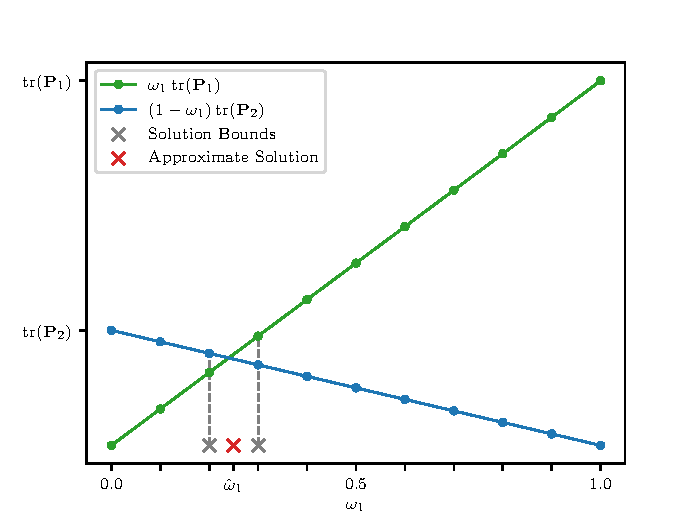
\includegraphics{figures/cloud_fusion_secfci_2sen_intersect.pdf}
    \end{center}
    \caption{Approximation of $\omega_1$ with stepsize $g=0.1$. Comparisons are only possible when $\omega_1$ is a multiple of $g$ (points on the graphs).}
    \label{fig:cloud_fusion:secfci_2sen_intersect}
    % TODO to figure. Y-axis should have 2 points, for trP1 and trP2. Omega^x should be omega_1. Make larger. Add a hat to the approximation of omega
 \end{figure}

In this way, computing fusion on the cloud homomorphically can be performed when having access to only local encryptions of information vectors and matrices, \eqref{eq:cloud_fusion:secfci_2sen_paillier_fuse_covs} and \eqref{eq:cloud_fusion:secfci_2sen_paillier_fuse_ests}, in addition to the sequences of order-revealing encryptions \eqref{eq:cloud_fusion:secfci_2sen_enc_seq_1} and \eqref{eq:cloud_fusion:secfci_2sen_enc_seq_2} that leak an approximation $\hat{\omega}_1 \approx \omega_1$.

% 
% ##    ##          ######  ######## ##    ## 
% ###   ##         ##    ## ##       ###   ## 
% ####  ##         ##       ##       ####  ## 
% ## ## ## #######  ######  ######   ## ## ## 
% ##  ####               ## ##       ##  #### 
% ##   ###         ##    ## ##       ##   ### 
% ##    ##          ######  ######## ##    ## 
% 

\subsection{Multi-sensor Case}\label{subsec:cloud_fusion:secfci_nsen}
To compute the fusion of $n$ sensor estimates in the information form we want the solutions to
\begin{equation}
    \mat{P}_{\mathsf{fus}}^{-1}\hat{\vec{x}}_{\mathsf{fus}} = \sum_{i=1}^n\omega_i\mat{P}_i^{-1}\hat{\vec{x}}_i
\end{equation}
and
\begin{equation}
    \mat{P}_{\mathsf{fus}}^{-1} = \sum_{i=1}^n\omega_i\mat{P}_i^{-1}\,.
\end{equation}
When the fusion weights $\omega_i$, $1\leq i\leq n$, $\sum_{i=1}^n\omega_i=1$, are known, we can again use the appropriate integer encoding and Paillier homomorphic properties to compute the fusion homomorphically as
\begin{equation}\label{eq:cloud_fusion:secfci_nsen_paillier_fuse_ests}
    \mathcal{E}_{\mathsf{pk}}\left(\mathsf{E}_1\left(\mat{P}_{\mathsf{fus}}^{-1}\hat{\vec{x}}_{\mathsf{fus}}\right)\right) \approx \oplus_{i=1}^n\left(\mathsf{E}_0(\omega_i)\otimes\mathcal{E}_{\mathsf{pk}}\left(\mathsf{E}_0\left(\mat{P}^{-1}_i\hat{\vec{x}}_i\right)\right)\right)
\end{equation}
and
\begin{equation}\label{eq:cloud_fusion:secfci_nsen_paillier_fuse_covs}
    \mathcal{E}_{\mathsf{pk}}\left(\mathsf{E}_1\left(\mat{P}_{\mathsf{fus}}^{-1}\right)\right) \approx \oplus_{i=1}^n\left(\mathsf{E}_0(\omega_i)\otimes\mathcal{E}_{\mathsf{pk}}\left(\mathsf{E}_0\left(\mat{P}^{-1}_i\right)\right)\right)\,.
\end{equation}
What remains is to compute the weights $\omega_i$ at the cloud such that the $n$-sensor FCI conditions \eqref{eq:prelims:fci_added_constraints} are met. Similar to the two-sensor case, we can use sequences of order-revealing encryptions to leak an approximation to this result. 

Each condition \eqref{eq:prelims:fci_added_constraints} is considered as a partial problem, that is,
\begin{equation}\label{eq:cloud_fusion:secfci_nsen_partial_sol_subspace}
    \omega_i\tr(\mat{P}_i) = \omega_{i+1}\tr(\mat{P}_{i+1})\,,
\end{equation}
with $1\leq i< n$ and $\sum_{i=1}^n\omega_i=1$, and their solution spaces, linear subspaces $\mathcal{S}_i$ over possible values of $\vec{\omega}=\begin{bsmallmatrix}\omega_1 & \cdots & \omega_n\end{bsmallmatrix}^\top$, desired. The intersection of these subspaces naturally results in the final solution to $\vec{\omega}$ in \eqref{eq:prelims:fci_matrix_equation}. Each solution space $\mathcal{S}_i$ can be defined by $n-1$ linearly independent solution points $\vec{\omega}_i^{(\zeta)}$, $1\leq \zeta\leq n-1$. $n-2$ of these solutions can be trivially obtained as the points where a single $\omega_j=1$, $j\neq i\neq i+1$ while the final point, $\vec{\omega}_i^{(n-1)}$, can be obtained as the solution to
\begin{equation}\label{eq:cloud_fusion:secfci_nsen_partial_sol_point}
    \omega_i\tr(\mat{P}_i) = (1-\omega_i)\tr(\mat{P}_{i+1})\,,
\end{equation}
$\omega_j=0$, $j\neq i\neq i+1$, noting equivalence to \eqref{eq:cloud_fusion:secfci_nsen_partial_sol_subspace} and $\omega_{i+1}=1-\omega_i$. The solutions $\vec{\omega}_i^{(\zeta)}$ and the $n-2$ dimensional subspace they define can be rewritten in parametric form as
\begin{equation}\label{eq:cloud_fusion:secfci_nsen_partial_subspace}
    \mathcal{S}_i(\vec{\gamma})=\vec{\omega}_i^{(1)} + 
    \begin{bmatrix}
        \bar{\vec{\omega}}_i^{(2)} & \cdots & \bar{\vec{\omega}}_i^{(n-1)}
    \end{bmatrix}
    \vec{\gamma}\,,
\end{equation}
where $\bar{\vec{\omega}}_i^{(\zeta)}=\vec{\omega}_i^{(\zeta)}-\vec{\omega}_i^{(1)}$ denote the direction vectors. The intersection of these $n-1$ subspaces gives the solution to $\vec{\omega}$ in \eqref{eq:prelims:fci_matrix_equation}. This solution, as well as the parameters for each subspace that provide it, $\vec{\gamma}_i$, can be obtained as a solution to the linear system
\begin{equation}\label{eq:cloud_fusion:secfci_nsen_omega_solution}
    \begin{bmatrix}
        -\mat{I} & \bar{\vec{\omega}}_1^{(2)} & \cdots & \bar{\vec{\omega}}_1^{(n-1)} & 0 & \cdots & 0\\
        \vdots & 0 &  & \ddots &  & \ddots & \vdots\\
        \vdots & \vdots & \ddots &  & \ddots &  & 0\\
        -\mat{I} & 0 & \cdots & 0 & \bar{\vec{\omega}}_{n-1}^{(2)} & \cdots & \bar{\vec{\omega}}_{n-1}^{(n-1)}
    \end{bmatrix}
    \begin{bmatrix}
        \vec{\omega}\\
        \vec{\gamma}_1\\
        \vdots\\
        \vec{\gamma}_{n-1}\\
    \end{bmatrix}=
    \begin{bmatrix}
        -\vec{\omega}_1^{(1)}\\
        \vdots\\
        -\vec{\omega}_{n-1}^{(1)}\\
    \end{bmatrix}\,.
\end{equation}

Therefore, to compute \eqref{eq:cloud_fusion:secfci_nsen_omega_solution} at the cloud leaking only comparisons required to compute the fusion weights, we approximate the solutions to \eqref{eq:cloud_fusion:secfci_nsen_partial_sol_point} with ORE sequences similar to the two-sensor case. Each sensor $i$ uses $\mathsf{sk}_{\mathsf{o}}$ to encrypt the discretisation 
\begin{equation}\label{eq:cloud_fusion:secfci_nsen_enc_seqs}
    \begin{split}
        \left\langle\mathcal{E}^{\mathsf{L}}_{\mathsf{sk}_{\mathsf{o}}}(0), \mathcal{E}^{\mathsf{L}}_{\mathsf{sk}_{\mathsf{o}}}(g\tr(\mat{P}_i)), \mathcal{E}^{\mathsf{L}}_{\mathsf{sk}_{\mathsf{o}}}(2g\tr(\mat{P}_i)),\dots,\mathcal{E}^{\mathsf{L}}_{\mathsf{sk}_{\mathsf{o}}}(\tr(\mat{P}_i))\right\rangle\,,\ & \text{if } i \text{ is odd, or}\\
        \left\langle\mathcal{E}^{\mathsf{R}}_{\mathsf{sk}_{\mathsf{o}}}(0), \mathcal{E}^{\mathsf{R}}_{\mathsf{sk}_{\mathsf{o}}}(g\tr(\mat{P}_i)), \mathcal{E}^{\mathsf{R}}_{\mathsf{sk}_{\mathsf{o}}}(2g\tr(\mat{P}_i)),\dots,\mathcal{E}^{\mathsf{R}}_{\mathsf{sk}_{\mathsf{o}}}(\tr(\mat{P}_i))\right\rangle\,,\ & \text{if } i \text{ is even,}
    \end{split}
\end{equation}
allowing for comparison between sequences from consecutive sensors $i$ and $i+1$. To approximate the solution to each \eqref{eq:cloud_fusion:secfci_nsen_partial_sol_point}, the sequence from sensor $i+1$ is reversed,
\begin{equation}\label{eq:cloud_fusion:secfci_nsen_enc_seqs_reversed}
    \begin{split}
        \left\langle\mathcal{E}^{\mathsf{L}}_{\mathsf{sk}_{\mathsf{o}}}(\tr(\mat{P}_i)),\mathcal{E}^{\mathsf{L}}_{\mathsf{sk}_{\mathsf{o}}}((1-g)\tr(\mat{P}_i)), \mathcal{E}^{\mathsf{L}}_{\mathsf{sk}_{\mathsf{o}}}((1-2g)\tr(\mat{P}_i)),\dots,\mathcal{E}^{\mathsf{L}}_{\mathsf{sk}_{\mathsf{o}}}(0)\right\rangle\,,\ & \text{if } i \text{ is odd, or}\\
        \left\langle\mathcal{E}^{\mathsf{R}}_{\mathsf{sk}_{\mathsf{o}}}(\tr(\mat{P}_i)), \mathcal{E}^{\mathsf{R}}_{\mathsf{sk}_{\mathsf{o}}}((1-g)\tr(\mat{P}_i)), \mathcal{E}^{\mathsf{R}}_{\mathsf{sk}_{\mathsf{o}}}((1-2g)\tr(\mat{P}_i)),\dots,\mathcal{E}^{\mathsf{R}}_{\mathsf{sk}_{\mathsf{o}}}(0)\right\rangle\,,\ & \text{if } i \text{ is even,}
    \end{split}
\end{equation}
resulting in sequences of the same form as \eqref{eq:cloud_fusion:secfci_2sen_enc_seq_1} and \eqref{eq:cloud_fusion:secfci_2sen_enc_seq_2}. The value $\hat{\omega}_i = \iota g + g/2 \approx \omega_i$, or in the case of an equality $\hat{\omega}_i = \iota g = \omega_i$, for some index $\iota$, is used to approximate the solution $\hat{\vec{\omega}}_i^{(n-1)} \approx \vec{\omega}_i^{(n-1)}$. A visualisation of solving \eqref{eq:cloud_fusion:secfci_nsen_omega_solution} with partial solutions \eqref{eq:cloud_fusion:secfci_nsen_partial_sol_point} in the three-sensor case is graphically shown in figure \ref{fig:cloud_fusion:secfci_nsen_partial_sols_and_intersect}.
\begin{figure}[htbp]
    \begin{subfigure}[htbp]{\textwidth}
        \begin{center}
            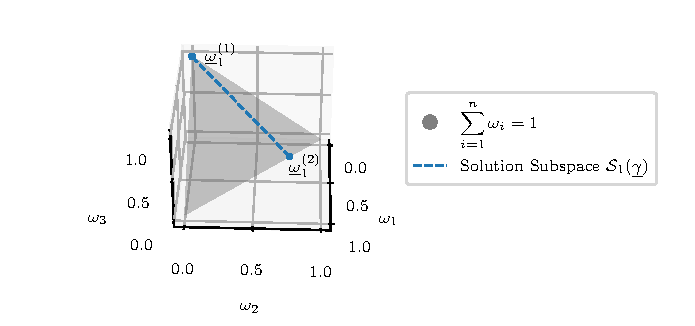
\includegraphics{figures/cloud_fusion_secfci_partial_sol_1.pdf}
        \end{center}
        \caption{Approximated solution space \eqref{eq:cloud_fusion:secfci_nsen_partial_subspace} when $i=1$.}
        \label{fig:cloud_fusion:secfci_partial_sol_1}
    \end{subfigure}
    \hfill
    \begin{subfigure}[htbp]{\textwidth}
        \begin{center}
            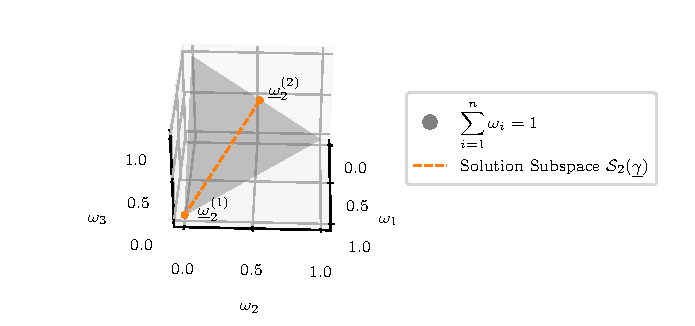
\includegraphics{figures/cloud_fusion_secfci_partial_sol_2.pdf}
        \end{center}
        \caption{Approximated solution space \eqref{eq:cloud_fusion:secfci_nsen_partial_subspace} when $i=2$.}
        \label{fig:cloud_fusion:secfci_partial_sol_2}
    \end{subfigure}
    \hfill
    \begin{subfigure}[htbp]{\textwidth}
        \begin{center}
            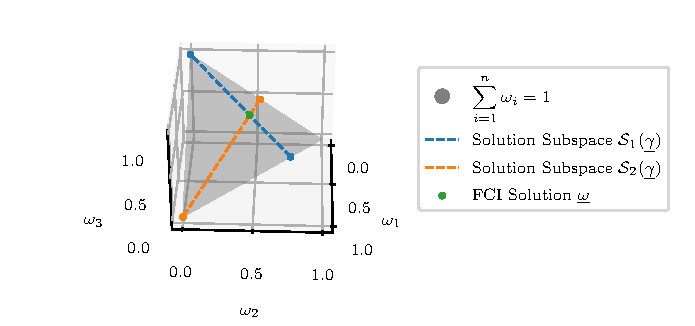
\includegraphics{figures/cloud_fusion_secfci_partial_sol_intersection.pdf}
        \end{center}
        \caption{Intersection of partial solutions spaces gives fusion weights $\vec{\omega}$ in \eqref{eq:prelims:fci_matrix_equation}.}
        \label{fig:cloud_fusion:secfci_partial_sol_intersection}
    \end{subfigure}
    \caption{Solving fusion weights $\vec{\omega}$ with approximations to \eqref{eq:cloud_fusion:secfci_nsen_partial_sol_point}.}
    \label{fig:cloud_fusion:secfci_nsen_partial_sols_and_intersect}
\end{figure}

A resulting estimate $\hat{\vec{\omega}} \approx \vec{\omega}$ can then be used with \eqref{eq:cloud_fusion:secfci_nsen_paillier_fuse_ests} and \eqref{eq:cloud_fusion:secfci_nsen_paillier_fuse_covs} to compute the fusion of $n$ information vectors and matrices at the cloud.

% 
%  ######   #######  ##     ## ########  
% ##    ## ##     ## ###   ### ##     ## 
% ##       ##     ## #### #### ##     ## 
% ##       ##     ## ## ### ## ########  
% ##       ##     ## ##     ## ##        
% ##    ## ##     ## ##     ## ##        
%  ######   #######  ##     ## ##        
% 

\subsection{Computational Complexity}\label{subsec:cloud_fusion:secfci_comp_complexity}
The method introduced allows the computation of FCI by using the Paillier and Lewi encryption schemes. Naturally, relying on encryption and homomorphic operations increases the complexity of computing this fusion at the sensor, cloud and querying party. Here, we look at the computational complexity of the method in terms of the required operations at each party. We assume that both the Lewi and Paillier schemes use the same key size, typically measured in bits, $\log{N}$, where $N$ is the Paillier modulus defined in section \ref{subsec:prelims:paillier}. In addition, we note the distinction between floating-point or small integer operations, treated as having runtime $O(1)$, and large integer operations with runtime dependent on bit length. While hardware architecture exists for faster encryption operations \cite{gueronIntelAdvancedEncryption2010}, we consider software implementations and treat large integer operations in terms of bit operations explicitly.

Individual encryption operation complexities with the assumptions made above have been summarised in table \ref{tab:cloud_fusion:secfci_op_complexity}. 
\begin{table}[htbp]
    \centering
    \caption{Computation complexity of involved encryption operations.}
    \label{tab:cloud_fusion:secfci_op_complexity}
    \begin{tabular}{|c|c|}
        \hline
        \textbf{Operation} & \textbf{Complexity} \\ 
        \hline
        Paillier Encryption & $O(\log^3{N})$ \\ 
        Paillier Decryption & $O(\log^3{N})$ \\ 
        Paillier Addition & $O(\log^2{N})$ \\ 
        Paillier Scalar Multiplication & $O(\log^3{N})$ \\ 
        Lewi \textit{Left} Encryption & $O(\log^2{N})$ \\ 
        Lewi \textit{Right} Encryption & $O(\log^2{N})$ \\ 
        Lewi Comparison & $O(\log^2{N})$ \\ 
        \hline
    \end{tabular}
\end{table}
Applying operation complexities to the fusion algorithm we get the computational complexity for the sensors, cloud and querying party. These can be seen in table \ref{tab:cloud_fusion:secfci_complexity}, where unencrypted FCI algorithm complexities are also shown for reference. 
\begin{table}[htbp]
   \centering
   \caption{Computation complexity for each party.}
   \label{tab:cloud_fusion:secfci_complexity}
   \begin{tabular}{|c|c|c|}
      \hline
       & \textbf{FCI} & \textbf{Confidential Fusion Leaking Weights} \\ 
      \hline
      Sensor & $O(1)$ & $O\left(d^2\log^3{N} + \frac{1}{g}\log^2{N}\right)$ \\ 
      Cloud & $O\left(nd^2+n^3\right)$ & $O\left(nd^2\log^3{N} + n\log{\frac{1}{g}} + n^3\right)$ \\ 
      Querying Party & $O(1)$ & $O\left(d^2\log^3{N}\right)$ \\ 
      \hline
   \end{tabular}
\end{table}
These complexities show the additional computational cost required for providing the security benefits of the presented scheme and must naturally be reflected in chosen hardware when developing a system where the benefits are desired.

% 
%  ######  ########  ######  
% ##    ## ##       ##    ## 
% ##       ##       ##       
%  ######  ######   ##       
%       ## ##       ##       
% ##    ## ##       ##    ## 
%  ######  ########  ######  
% 

\subsection{Security Analysis}\label{subsec:cloud_fusion:secfci_security}
Recalling the cryptographic aims of the estimate fusion problem introduced in the problem formulation and weakened for the presented method, we desire estimate information to be encrypted with a notion meeting IND-CPA at the fusion cloud and eavesdroppers while allowing the leakage of fusion weights, and naturally any functions derivable only from this information.

Since Paillier encryptions \eqref{eq:cloud_fusion:secfci_nsen_paillier_fuse_ests} and \eqref{eq:cloud_fusion:secfci_nsen_paillier_fuse_covs} meet the IND-CPA notion, this information meets the desired aims. The remaining available information to the cloud and eavesdroppers are the sequences encrypted by the Lewi ORE scheme. This scheme meets the simulation-based security discussed in section \ref{subsec:prelims:lewi_ore} and is shown in section \ref{subsec:cloud_fusion:secfci_nsen} to correspond to the leakage of approximations to the weights $\omega_i$, in addition to some leakage beyond the used ciphertext order comparisons due to the relaxation of the IND-OCPA notation (which can be difficult to quantify in context). Lastly, we also acknowledge an implicit leakage of estimate dimension $d$ associated with the use of elementwise encryption. Although methods for homomorphic encryption of vectors exist \cite{alexandruPrivateWeightedSum2020}, we leave this as future work on this topic and note that the dimension $d$ may leak information about the data fusion use case but that estimates themselves remain encrypted.

The leakages present in the introduced method, namely the leakage of fusion weights and estimate dimensions, may lead to inferences about sensor hardware and must naturally be considered when planning the implementation of this method in a real-world system.

% 
%  ######  #### ##     ## 
% ##    ##  ##  ###   ### 
% ##        ##  #### #### 
%  ######   ##  ## ### ## 
%       ##  ##  ##     ## 
% ##    ##  ##  ##     ## 
%  ######  #### ##     ## 
% 

\subsection{Simulation}\label{subsec:cloud_fusion:secfci_simulation}
Along with the discussions above, we have implemented a simulation of the method to demonstrate its fusion accuracy when compared to the FCI algorithm on a trusted cloud. A constant-velocity linear system, 
\begin{equation}\label{eq:cloud_fusion:secfci_system_model}
    \vec{x}_{k+1} = 
    \begin{bmatrix}
        1 & 0 & 0.5 & 0\\
        0 & 1 & 0   & 0.5\\
        0 & 0 & 1   & 0\\
        0 & 0 & 0   & 1
    \end{bmatrix}\vec{x}_k + \vec{w}_k\,,
\end{equation}
with noise term
\begin{equation}
    \vec{w}_k\sim\mathcal{N}\left(\vec{0},\ \frac{1}{10^{3}}\cdot
    \begin{bmatrix}
        0.42 & 0    & 1.25 & 0\\
        0    & 0.42 & 0    & 1.25\\
        1.25 & 0    & 5.0  & 0\\
        0    & 1.25 & 0    & 5.0
    \end{bmatrix}
    \right)\,,
\end{equation}
was simulated and measured by four independent position sensors $1\leq i\leq 4$, that produced measurements 
\begin{equation}\label{eq:cloud_fusion:secfci_measurement_model}
    \vec{z}_{k,i} = 
    \begin{bmatrix}
        1 & 0 & 0 & 0\\
        0 & 1 & 0 & 0
     \end{bmatrix}\vec{x}_k + \vec{v}_{k,i}\,,\qquad \vec{v}_{k,i}\sim\mathcal{N}\left(\vec{0},\mat{R}_i\right)\,,
\end{equation}
with noise term covariances sampled independently, resulting in
\begin{equation}\label{eq:cloud_fusion:secfci_measurement_model_covariances}
    \begin{split}
        &\mat{R}_1 = 
        \begin{bmatrix}
            4.77 & -0.15\\
            -0.15 & 4.94
        \end{bmatrix}\,,\\
        &\mat{R}_2 = 
        \begin{bmatrix}
            2.99 & -0.55\\
            -0.55 & 4.44
        \end{bmatrix}\,,\\
        &\mat{R}_3 = 
        \begin{bmatrix}
            2.06 & 0.68\\
            0.68 & 1.96
        \end{bmatrix}\text{ and }\\
        &\mat{R}_4 = 
        \begin{bmatrix}
            1.17 & 0.80\\
            0.80 & 0.64
        \end{bmatrix}\,.
    \end{split}
\end{equation}
Each sensor ran a local linear Information Filter (IF) from section \ref{subsec:prelims:if}, initialised with the true state of the system, before processing and sending its estimate information, $\mat{P}_{k, i}^{-1}\hat{\vec{x}}_{k, i}$ and $\mat{P}_{k, i}^{-1}$, to the cloud for fusion. At each timestep, the time-independent fusion of information vectors and matrices was computed homomorphically at the cloud and decrypted by the querying party. The simulation was written in the Python and C programming languages, using the PHE Paillier encryption scheme library \cite{PythonPaillier2013}, and using a key size of $512$ bits for encryption schemes. Figure \ref{fig:cloud_fusion:secfci_sim_error} shows the average estimation error of $1000$ simulations when using our algorithm with varying stepsizes $g$ alongside the standard FCI algorithm. 
\begin{figure}[htbp]
    \centering
    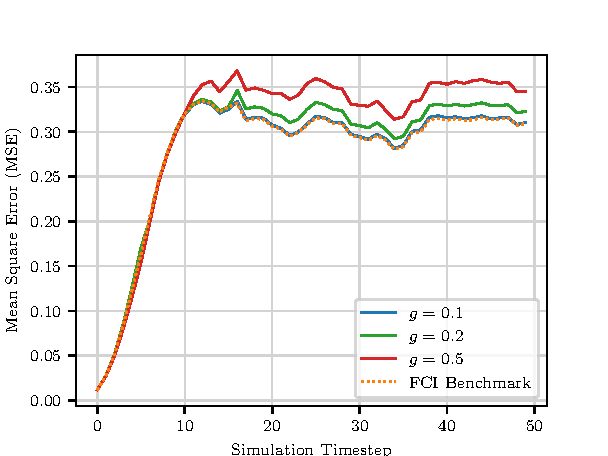
\includegraphics{figures/cloud_fusion_secfci_sim_error.pdf}
    \caption{Average MSE with varying stepsize $g$ over $1000$ simulation runs.}
    \label{fig:cloud_fusion:secfci_sim_error}
 \end{figure}
 In all cases, resulting plaintext information vectors and matrices were converted to estimates and estimate error covariances before comparison with the true simulated state. From the figure, it can be seen that the estimation error of our method is similar to the normal FCI method when stepsize $g$ is small, $g=0.1$, but grows as expected when $g$, and thus the possible error in weights $\omega_i$ is increased.

Since the system described by \eqref{eq:cloud_fusion:secfci_system_model}, \eqref{eq:cloud_fusion:secfci_measurement_model} and estimated by the IF reaches an estimation steady-state, fusion weights $\omega_i$ do as well. Figure \ref{fig:cloud_fusion:secfci_omega_error} shows the steady state error of estimated weights when compared to the true FCI weights. 
\begin{figure}[htbp]
    \centering
    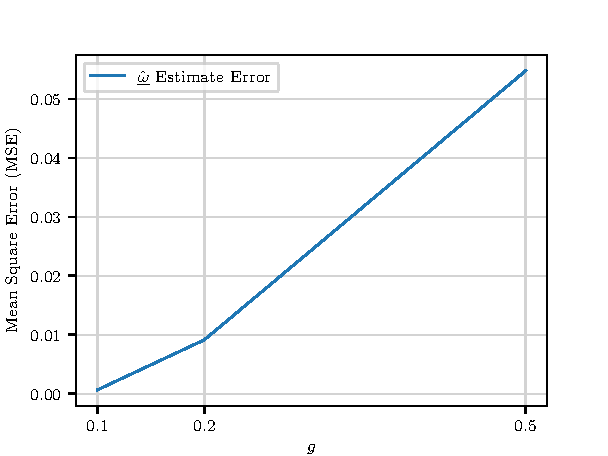
\includegraphics{figures/cloud_fusion_secfci_omega_error.pdf}
    \caption{Steady-state MSE of estimated weights $\hat{\vec{\omega}}$ with varying stepsize $g$.}
    \label{fig:cloud_fusion:secfci_omega_error}
\end{figure}
Here, the maximum errors in fusion weights naturally depend on the stepsize $g$ and support the results seen in figure \ref{fig:cloud_fusion:secfci_sim_error}. Further, an upper bound on this error can be derived by considering the maximum error of each approximation \eqref{eq:cloud_fusion:secfci_nsen_partial_sol_point} and is given by
\begin{equation}
    \left|\hat{\vec{\omega}} - \vec{\omega}\right| \leq \frac{g}{2}\sqrt{n}\,.
\end{equation}

% 
% 8888888888 888     888  .d8888b. 8888888 .d88888b.  888b    888      888b    888 888      
% 888        888     888 d88P  Y88b  888  d88P" "Y88b 8888b   888      8888b   888 888      
% 888        888     888 Y88b.       888  888     888 88888b  888      88888b  888 888      
% 8888888    888     888  "Y888b.    888  888     888 888Y88b 888      888Y88b 888 888      
% 888        888     888     "Y88b.  888  888     888 888 Y88b888      888 Y88b888 888      
% 888        888     888       "888  888  888     888 888  Y88888      888  Y88888 888      
% 888        Y88b. .d88P Y88b  d88P  888  Y88b. .d88P 888   Y8888      888   Y8888 888      
% 888         "Y88888P"   "Y8888P" 8888888 "Y88888P"  888    Y888      888    Y888 88888888 
%                                                                                           
%                                                                                           
%                                                                                           
% 

\section{Confidential Cloud Fusion Without Leaking Fusion Weights}\label{sec:cloud_fusion:secfci2}
Previously, we presented a method for solving the estimate fusion problem by weakening the desired cryptographic aims in section \ref{sec:cloud_fusion:problem}. In this section, we present a method that meets these aims exactly by making a relaxation on the produced fusion output of the fusion cloud.
\begin{description}
    \item[Broader fusion output] In this method, the fusion cloud is not strictly required to produce the fused information vector $\mat{P}_{\mathsf{fus}}^{-1}\hat{\vec{x}}_{\mathsf{fus}}$ and matrix $\mat{P}_{\mathsf{fus}}^{-1}$. Instead, any statistics over data from individual sensors $i$ can be computed homomorphically at the fusion cloud and provided to the querying party. For example, the sum statistic over inverted estimate covariance traces, $\sum_{i=1}^n \tr(\mat{P}_i)^{-1}$, may be returned.
\end{description}

The idea behind the method is to postpone the evaluation of operations that cannot be performed homomorphically until partial fusion results are decrypted by the querying party. The remaining operations are then evaluated on unencrypted inputs to produce the final fusion results. First, we note that FCI fusion \eqref{eq:prelims:ci_info_vec}, \eqref{eq:prelims:ci_info_mat} and \eqref{eq:prelims:fci_solution} can be rearranged and weights substituted to obtain
\begin{equation}\label{eq:cloud_fusion:secfci2_info_vec_rearrange}
    \mat{P}_{\mathsf{fus}}^{-1}\hat{\vec{x}}_{\mathsf{fus}} = \left(\sum_{i=1}^n \frac{1}{\tr(\mat{P}_i)}\right)^{-1}\sum_{i=1}^n\frac{1}{\tr(\mat{P}_i)}\mat{P}_i^{-1}\hat{\vec{x}}_i
\end{equation}
and
\begin{equation}\label{eq:cloud_fusion:secfci2_info_mat_rearrange}
    \mat{P}_{k,\mathsf{fus}}^{-1} = \left(\sum_{i=1}^n \frac{1}{\tr(\mat{P}_i)}\right)^{-1}\sum_{i=1}^n \frac{1}{\tr(\mat{P}_i)}\mat{P}_i^{-1}\,.
\end{equation}

In this form, innermost summations  
\begin{equation}
    \sum_{i=1}^n \frac{1}{\tr(\mat{P}_i)}\,,\ \sum_{i=1}^n \frac{1}{\tr(\mat{P}_i)}\mat{P}_i^{-1}\text{ and }\sum_{i=1}^n\frac{1}{\tr(\mat{P}_i)}\mat{P}_i^{-1}\hat{\vec{x}}_i
\end{equation}
combine information from individual sensors $i$, are computable homomorphically given suitable encryption and suit the fusion relaxation defined above. Encryptions of these sums can then be decrypted by the querying party, before remaining inversions and multiplications in \eqref{eq:cloud_fusion:secfci2_info_vec_rearrange} and \eqref{eq:cloud_fusion:secfci2_info_mat_rearrange} can be computed to obtain the final results. To depict this straightforward process, pseudocode for the encryption at the sensors, fusion at the cloud and decryption at the querying party are shown in algorithms \ref{alg:cloud_fusion:secfci2_sensor_steps}, \ref{alg:cloud_fusion:secfci2_cloud_steps} and \ref{alg:cloud_fusion:secfci2_query_steps}, respectively. As in the previous section, the Paillier encryption scheme, producing keys $\mathsf{pk}$ and $\mathsf{sk}$, is used, encoding from section \ref{subsec:prelims:encoding} is used with $M=N$, where $N$ is the Paillier scheme modulus, and an appropriate precision $\phi$ is chosen.
\begin{algorithm}[htbp]
\caption{Encryption at the Sensors}\label{alg:cloud_fusion:secfci2_sensor_steps}
\begin{algorithmic}[1]
    \setstretch{1.35}
    \Procedure{Estimate}{$i$, $\mathsf{pk}$}
    \State Estimate $\mat{P}_i^{-1}\hat{\vec{x}}_i$ locally
    \State Estimate $\mat{P}_i^{-1}$ locally
    \LineComment{Encode and encrypt scaling, covariance and estimate components}
    \State $\xi_i \gets \mathcal{E}_{\mathsf{pk}}\left(\mathsf{E}_{0}\left(\frac{1}{\tr(\mat{P}_i)}\right)\right)$
    \State $\vec{b}_i \gets \mathcal{E}_{\mathsf{pk}}\left(\mathsf{E}_{0}\left(\frac{1}{\tr(\mat{P}_i)}\mat{P}_i^{-1}\hat{\vec{x}}_i\right)\right)$
    \State $\mat{B}_i \gets \mathcal{E}_{\mathsf{pk}}\left(\mathsf{E}_{0}\left(\frac{1}{\tr(\mat{P}_i)}\mat{P}_i^{-1}\right)\right)$
    \State Send $\xi_i$, $\vec{b}_i$ and $\mat{B}_i$ to fusion cloud
    \EndProcedure
\end{algorithmic}
\end{algorithm}
\begin{algorithm}[htbp]
\caption{Partial Fusion at the Cloud}\label{alg:cloud_fusion:secfci2_cloud_steps}
\begin{algorithmic}[1]
    \setstretch{1.35}
    \Procedure{PartialFuse}{$\mathsf{pk}$}
    \State Receive $\xi_i$, $\vec{b}_i$ and $\mat{B}_i$ for all $1\leq i \leq n$
    \LineComment{Perform homomorphic summations}
    \State $\xi \gets \oplus_{i=1}^{n} \xi_i$
    \State $\vec{b} \gets \oplus_{i=1}^{n} \vec{b}_i$
    \State $\mat{B} \gets \oplus_{i=1}^{n} \mat{B}_i$
    \State Store $\xi$, $\vec{b}$ and $\mat{B}$ in case of query
    \EndProcedure
\end{algorithmic}
\end{algorithm}
\begin{algorithm}[htbp]
\caption{Completing Fusion at the Querying Party}\label{alg:cloud_fusion:secfci2_query_steps}
\begin{algorithmic}[1]
    \setstretch{1.35}
    \Procedure{QueryFuse}{$\mathsf{pk}$, $\mathsf{sk}$}
    \State Query and receive $\xi$, $\vec{b}$ and $\mat{B}$ from fusion cloud
    \LineComment Decrypt and decode
    \State $\bar{\xi} \gets \mathsf{E}^{-1}_{0}\left(\mathcal{D}_{\mathsf{pk},\mathsf{sk}}\left(\xi\right)\right)$
    \State $\bar{\vec{b}} \gets \mathsf{E}^{-1}_{0}\left(\mathcal{D}_{\mathsf{pk},\mathsf{sk}}\left(\vec{b}\right)\right)$
    \State $\bar{\mat{B}} \gets \mathsf{E}^{-1}_{0}\left(\mathcal{D}_{\mathsf{pk},\mathsf{sk}}\left(\mat{B}\right)\right)$
    \LineComment Compute remaining fusion operations
    \State $\mat{P}_{\mathsf{fus}}^{-1}\hat{\vec{x}}_{\mathsf{fus}} \gets \bar{\xi}^{-1} \cdot \bar{\vec{b}}$
    \State $\mat{P}_{\mathsf{fus}}^{-1} \gets \bar{\xi}^{-1} \cdot \bar{\mat{B}}$
    \State \Return $\mat{P}_{\mathsf{fus}}^{-1}\hat{\vec{x}}_{\mathsf{fus}}$, $\mat{P}_{\mathsf{fus}}^{-1}$
    \EndProcedure
\end{algorithmic}
\end{algorithm}

Along with allowing the summations to be performed homomorphically on the cloud, we note that this form of the FCI also allows the cloud's partial fusion operations to be evaluated sequentially. This can be seen in algorithm \ref{alg:cloud_fusion:secfci2_cloud_steps}, where individual components $\xi_i$, $\vec{b}_i$ and $\mat{B}_i$ from each sensor can continue to be sequentially aggregated as sensors send their estimate information. This, in turn, supports the dynamic joining and leaving of sensors in the network without affecting the cloud or the operations of the querying party.

% 
%  ######   #######  ##     ## ########  
% ##    ## ##     ## ###   ### ##     ## 
% ##       ##     ## #### #### ##     ## 
% ##       ##     ## ## ### ## ########  
% ##       ##     ## ##     ## ##        
% ##    ## ##     ## ##     ## ##        
%  ######   #######  ##     ## ##        
% 

\subsection{Computational Complexity}\label{subsec:cloud_fusion:secfci2_comp_complexity}
As with the previous method, we allow the homomorphic computation of FCI fusion at the computational cost of encryption and homomorphic operations. Here, we look at this additional cost for each involved party using the newly presented scheme. We again assume floating-point and small integer operations to have complexity $O(1)$, the Paillier scheme to have key size $\log{N}$ bits and repeat the Paillier operation complexities in table \ref{tab:cloud_fusion:secfci2_op_complexity} for convenience. 
\begin{table}[htbp]
    \centering
    \caption{Computation complexity of Paillier encryption operations.}
    \label{tab:cloud_fusion:secfci2_op_complexity}
    \begin{tabular}{|c|c|}
        \hline
        \textbf{Operation} & \textbf{Complexity} \\ 
        \hline
        Paillier Encryption & $O(\log^3{N})$ \\ 
        Paillier Decryption & $O(\log^3{N})$ \\ 
        Paillier Addition & $O(\log^2{N})$ \\ 
        Paillier Scalar Multiplication & $O(\log^3{N})$ \\ 
        \hline
    \end{tabular}
\end{table}
In table \ref{tab:cloud_fusion:secfci2_complexity}, we apply the Paillier operation complexities to the presented method and the unencrypted FCI algorithm is again shown for reference.
\begin{table}[htbp]
    \centering
    \caption{Computation complexity for each party.}
    \label{tab:cloud_fusion:secfci2_complexity}
    \begin{tabular}{|c|c|c|}
       \hline
        & \textbf{FCI} & \textbf{Confidential Fusion} \\ 
       \hline
       Sensor & $O(1)$ & $O\left(d^2\log^3{N}\right)$ \\ 
       Cloud & $O\left(nd^2 + n^3\right)$ & $O\left(nd^2\log^2{N}\right)$ \\ 
       Querying Party & $O(1)$ & $O\left(d^2\log^3{N}\right)$ \\ 
       \hline
    \end{tabular}
 \end{table}
Here we see that the burden of computation is reduced when compared to the method leaking weights in section \ref{sec:cloud_fusion:secfci}. This can be attributed to no longer requiring the Lewi ORE scheme and the computational simplicity of the final fusion steps at the querying party compared to the required decryption operations. These computational requirements are a necessity for providing the specified security and fusion aims and must be considered when choosing hardware for a physical system where the aims are desired.

% 
%  ######  ########  ######  
% ##    ## ##       ##    ## 
% ##       ##       ##       
%  ######  ######   ##       
%       ## ##       ##       
% ##    ## ##       ##    ## 
%  ######  ########  ######  
% 

\subsection{Security Analysis}\label{subsec:cloud_fusion:secfci2_security}
Showing that the cryptographic aims of the fusion problem are met is relatively straightforward. Our aim is for all estimate information, excluding locally produced estimates, that is available to the cloud, eavesdroppers and sensors to be encrypted with a scheme meeting the IND-CPA notion. Since the Paillier scheme meets this notion and all transmitted information is encrypted, and noting that the cloud, estimators and eavesdroppers do not hold the secret key $\mathsf{sk}$, the cryptographic aim is met. We do, however, note that the implicit leakage of state dimension $d$ is again present in this method due to the reliance on elementwise encryption.

Lastly, when discussing security, we recall that the partial computation of FCI in this method supports the dynamic joining and leaving of sensors during fusion, but note that the implementation of this in practice introduces additional implicit leakages that need to be considered. Periodic estimation from a sensor may reveal when the sensor is within an estimation range or context, potentially leaking sensor privacy. To combat this, appropriate methods to mitigate implicit leakage need to be considered for real hardware, for example, sending dummy estimate information, $\mathcal{E}_{\mathsf{pk}}(\mathsf{E}_0(0))$, $\mathcal{E}_{\mathsf{pk}}(\mathsf{E}_0(\mat{0}))$ and $\mathcal{E}_{\mathsf{pk}}(\mathsf{E}_0(\vec{0}))$, when sensor $i$ is out of estimation context.

% 
%  ######  #### ##     ## 
% ##    ##  ##  ###   ### 
% ##        ##  #### #### 
%  ######   ##  ## ### ## 
%       ##  ##  ##     ## 
% ##    ##  ##  ##     ## 
%  ######  #### ##     ## 
% 

\subsection{Simulation}\label{subsec:cloud_fusion:secfci2_simulation}
To demonstrate the accuracy of the method and compare it to the method in section \ref{sec:cloud_fusion:secfci} as well as the FCI algorithm it approximates, we have implemented a simulation of the fusion scenario. Since errors in fusion are now only introduced during real number quantisation we expect the estimation error to be smaller than that in section \ref{sec:cloud_fusion:secfci}. Code was written in the Python programming language, again using the PHE Paillier encryption scheme library \cite{PythonPaillier2013}. A key size of $512$ bits was used, and the constant-velocity linear model in \eqref{eq:cloud_fusion:secfci_system_model} was implemented. At each timestep $k$, the system state $\vec{x}_k$ was measured by $m=4$ sensors, $1\leq i \leq 4$, with measurements $\vec{z}_{k,i}$ following the measurement models \eqref{eq:cloud_fusion:secfci_measurement_model} and covariances \eqref{eq:cloud_fusion:secfci_measurement_model_covariances}. Using a linear IF, initialised with the true state of the system, each sensor produced estimate information $\mat{P}_{k, i}^{-1}\hat{\vec{x}}_{k, i}$ and $\mat{P}_{k, i}^{-1}$, respectively, that were processed, encrypted and fused at the cloud and querying party. The fusion error results of $1000$ simulation runs are shown in figure \ref{fig:cloud_fusion:secfci2_sim_error}. 
\begin{figure}[htbp]
    \centering
    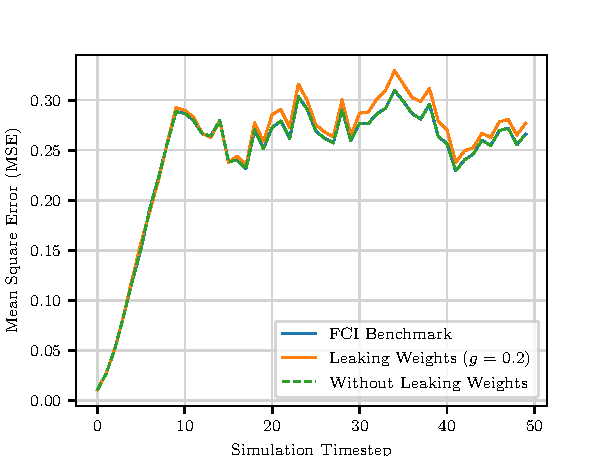
\includegraphics{figures/cloud_fusion_secfci2_sim_error.pdf}
    \caption{Average MSE of presented fusion methods over $1000$ simulations.}
    \label{fig:cloud_fusion:secfci2_sim_error}
\end{figure}
From the figure, we can see the expected similarity in performance between all three methods. The better approximation of the fusion weights in the method from this section results in slightly more accurate results than those with the method from section \ref{sec:cloud_fusion:secfci}, however, choosing a smaller stepsize $g$ can reduce this difference, albeit increase complexity.

% 
%  .d8888b.   .d88888b.  888b    888  .d8888b.  
% d88P  Y88b d88P" "Y88b 8888b   888 d88P  Y88b 
% 888    888 888     888 88888b  888 888    888 
% 888        888     888 888Y88b 888 888        
% 888        888     888 888 Y88b888 888        
% 888    888 888     888 888  Y88888 888    888 
% Y88b  d88P Y88b. .d88P 888   Y8888 Y88b  d88P 
%  "Y8888P"   "Y88888P"  888    Y888  "Y8888P"  
%                                               
%                                               
%                                               
% 

\section{Conclusions on Confidential Estimate Fusion}\label{sec:cloud_fusion:conclusion}
In this chapter, we have presented two methods for approximating the FCI fusion algorithm on an untrusted cloud where estimates and final fusion meet specified cryptographic aims. The methods primarily differ in whether the FCI fusion weights are leaked to eavesdroppers and the cloud as well as the assumptions on collusions between parties in the network.

The first method, providing confidential fusion with the leakage of weights, introduced in section \ref{sec:cloud_fusion:secfci}, has the benefit of allowing the untrusted cloud to prioritise sensors when performing fusion. This is done by preferring sensors that reduce fused estimate error, as indicated by their fusion weight, but requires the assumption that sensors are trusted and cannot collude maliciously. The method also requires the use of two encryption schemes, resulting in higher computational complexity at sensors and the cloud, as can be seen in section \ref{subsec:cloud_fusion:secfci_comp_complexity}. The second method, presented in section \ref{sec:cloud_fusion:secfci2}, provides confidential fusion without the leakage of weights. This method doesn't consider sensors as trusted parties and leaks no information beyond the implicit leakage of state dimension, present in both methods. The stronger security guarantees come with disadvantages, namely that the cloud cannot prioritise estimates based on their fusion error and that an additional, albeit constant, complexity is present at the querying party. Both methods have their computational complexity and security implications analysed and are simulated to demonstrate estimation performance.

Future directions for the topic of confidential data fusion include multi-variable encryption, removing the implicit leakage of state dimension and the extension of the method to decentralised environments where confidential fusion without a centralised cloud is desirable.
